\documentclass[11pt,oneside]{book}
%\documentclass{exam}
\usepackage[margin=1in]{geometry}
\usepackage[T1]{fontenc}
\usepackage[utf8]{inputenc}
\usepackage{microtype}
\usepackage{graphicx, caption, lipsum}
%\usepackage{hyperref}
\usepackage{graphicx}
\usepackage{amsmath}
\usepackage{multicol}
\usepackage{caption}
\usepackage{amsthm}
\usepackage{tasks}
\usepackage{amsmath, amssymb, amsthm}
\usepackage{xcolor}
\usepackage[most]{tcolorbox}
\usepackage{float}  
\usepackage{hyperref}
\renewcommand{\epsilon}{\varepsilon}
\everymath{\displaystyle}


% --- Custom Colors matching the screenshot ---
\definecolor{defgreen}{RGB}{46, 125, 50}
\definecolor{defgreenbg}{RGB}{241, 248, 242}

\definecolor{exblue}{RGB}{30, 100, 200}
\definecolor{exbluebg}{RGB}{240, 244, 250}

\definecolor{thmred}{RGB}{180, 60, 20}
\definecolor{thmredbg}{RGB}{253, 245, 240}

\definecolor{thmpurple}{RGB}{150, 50, 200}
\definecolor{thmpurplebg}{RGB}{250, 240, 255}

% --- Base tcolorbox style for left-bar boxes ---
\tcbset{
  leftbarbox/.style={
    enhanced,
    breakable,                  % Allows boxes to split across page breaks
    frame hidden,               % Hides standard rectangular frame
    sharp corners,
    boxrule=0pt,
    left=8pt, right=8pt, top=6pt, bottom=6pt,
    borderline west={3pt}{0pt}{#1}, % Creates the colored left vertical stripe
  }
}

% --- Environment Declarations ---

% 1. Definition (Green)
\newtcolorbox[auto counter, number within=chapter]{definition}[1][]{
  leftbarbox=defgreen,
  colback=defgreenbg,
  title={\textcolor{defgreen}{\textbf{Definition \thetcbcounter\ \ifstrempty{#1}{}{(#1).}}}},
  detach title,
  before upper={\tcbtitle\ }
}

% 2. Example (Blue - Unnumbered option shown in screenshot)
\newtcolorbox{example}[1][]{
  leftbarbox=exblue,
  colback=exbluebg,
  title={\textcolor{exblue}{\textbf{Example\ifstrempty{#1}{}{ (#1)}.\ }}},
  detach title,
  before upper={\tcbtitle}
}

% 3. Lemma / Theorem (Brown / Orange)
\newtcolorbox[auto counter, number within=chapter]{lemma}[1][]{
  leftbarbox=thmred,
  colback=thmredbg,
  title={\textcolor{thmred}{\textbf{Lemma \thetcbcounter\ \ifstrempty{#1}{}{(#1).}}}},
  detach title,
  before upper={\tcbtitle\ }
}         

% --- Color Definitions ---
\definecolor{workblack}{RGB}{20, 20, 20}
\definecolor{workgraybg}{RGB}{245, 245, 245}

% --- Worked Example Box ---
\newtcolorbox[auto counter, number within=chapter]{workedexample}[1][]{
  leftbarbox=workblack,
  colback=workgraybg,
  title={\textcolor{workblack}{\textbf{Worked Example \thetcbcounter\ \ifstrempty{#1}{}{(#1).}}}},
  detach title,
  before upper={\tcbtitle\ }
}

% --- Exercise Box ---
\newtcolorbox[auto counter, number within=chapter]{exercise}[1][]{
  leftbarbox=thmpurple,
  colback=thmpurplebg,
  title={\textcolor{thmpurple}{\textbf{Exercise \thetcbcounter\ \ifstrempty{#1}{}{(#1).}}}},
  detach title,
  before upper={\tcbtitle\ }
}

% ============================================================================

\begin{document}

\begin{definition}[Limit as $x \to \infty$]
    Let $f$ be defined on $\left[ c, \infty \right)$ for some $c\in\mathbb{R}$ We say that $\lim_{x \to \infty} f(x) = L$ if for each $\epsilon > 0$ there exists a corresponding $M > 0$ such that for all $x > M$, we have
    \[ \left| f(x) - L \right| < \epsilon \]
\end{definition}

\begin{figure}[H]
    \centering
    \caption{Visual representation of the definition of $\lim_{x \to \infty} f(x) = L$}
    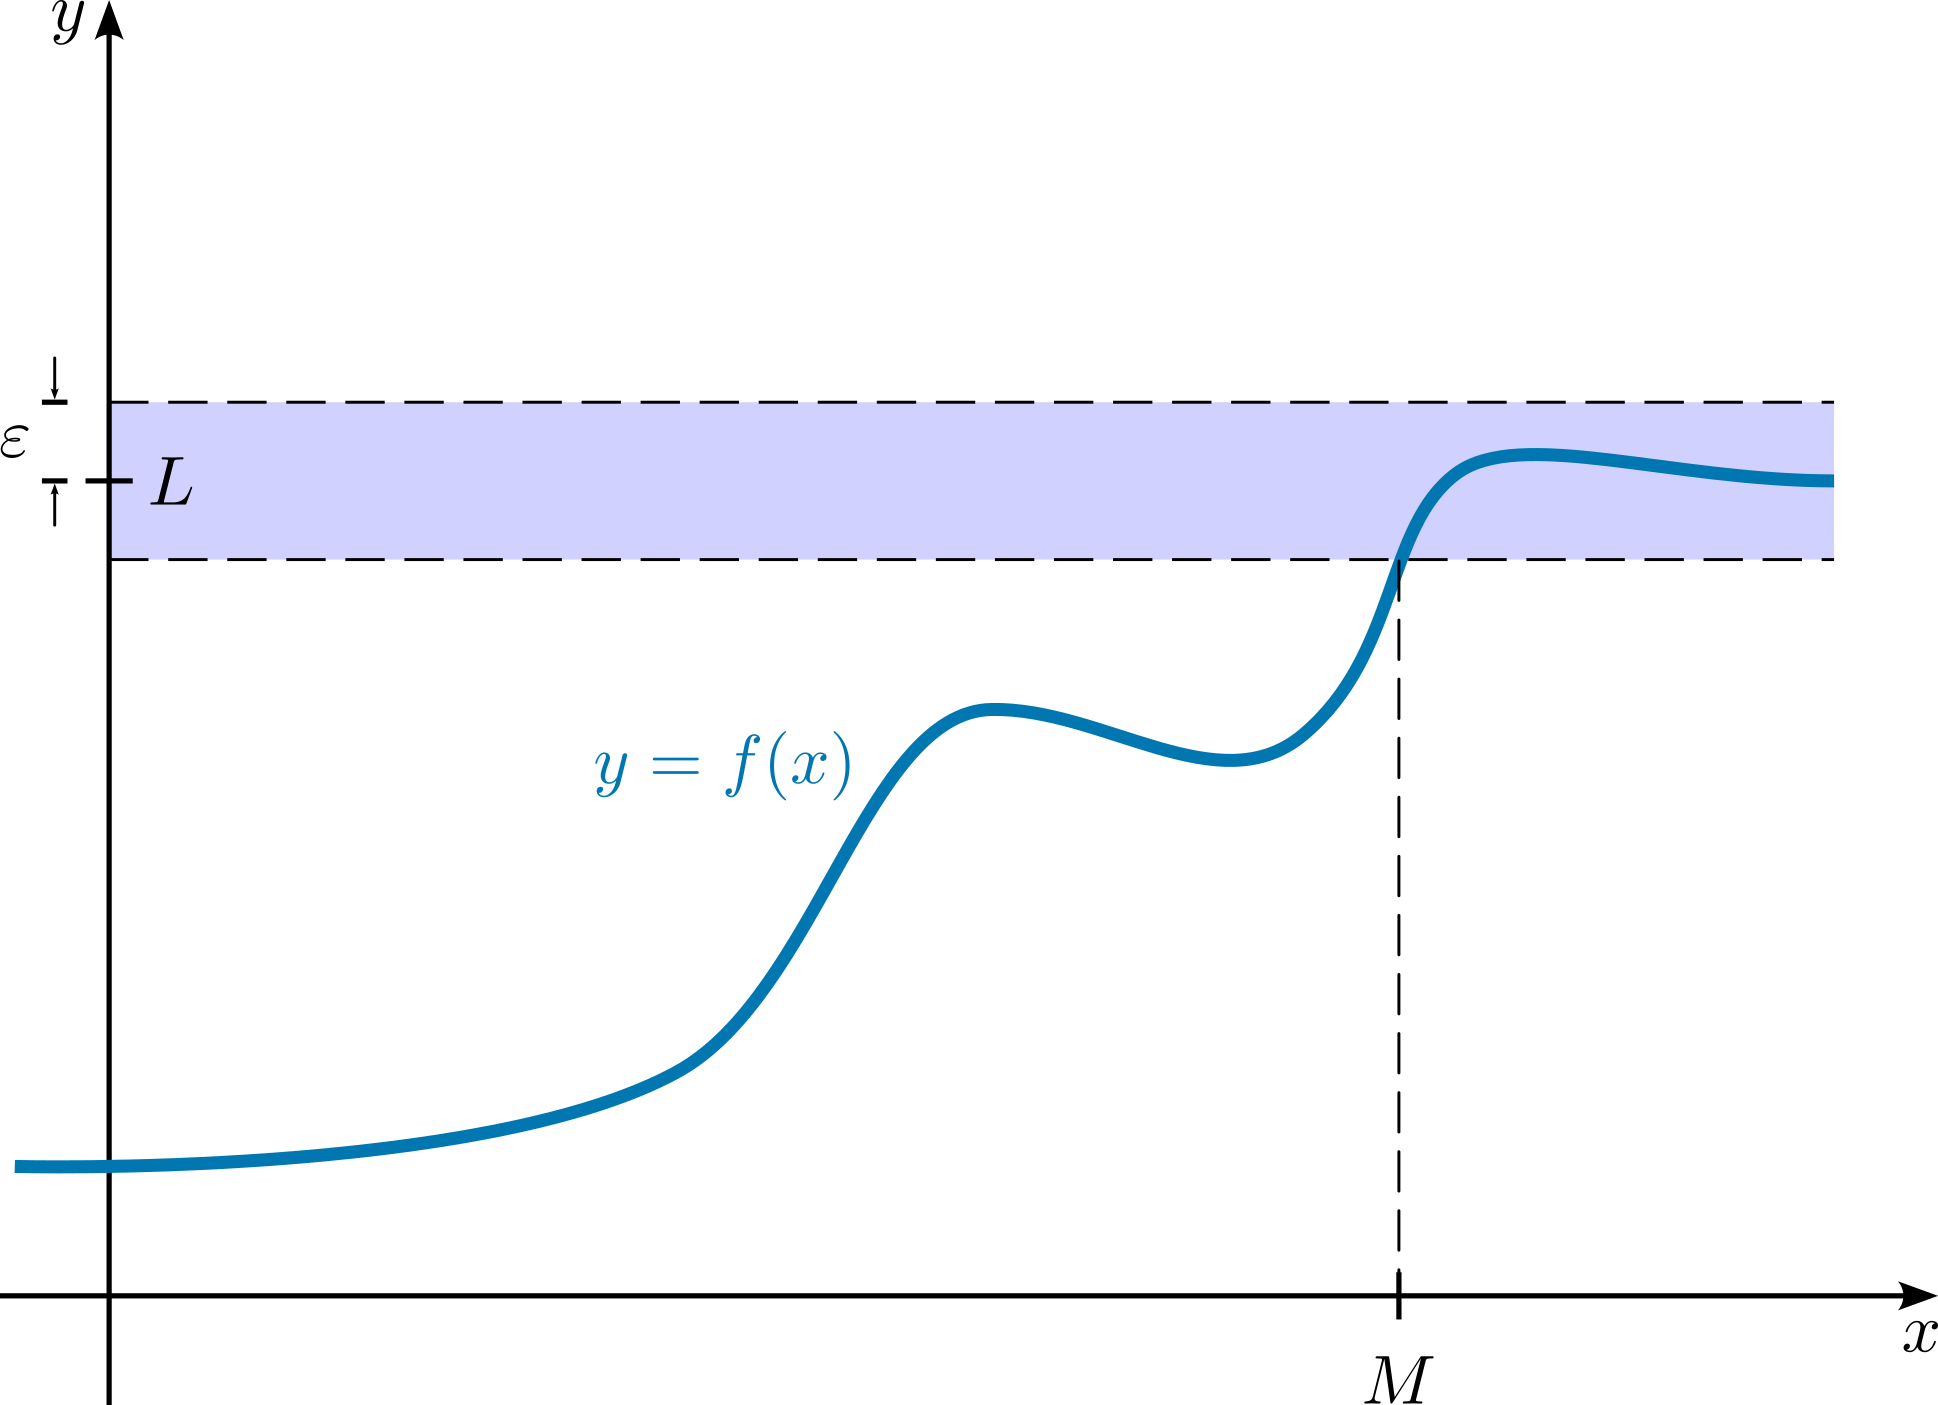
\includegraphics[width=0.35\linewidth]{limits_at_infinity.png}
\end{figure}

\begin{example}
  Consider the function $f(x) = \frac{1}{x}$ for $x > 0$. We want to show that $\lim_{x \to \infty} f(x) = 0$.  \newline\vspace{8pt}
  \textbf{Proof: } Let $\epsilon>0$ and choose $M = \frac{1}{\sqrt{\epsilon}}$. Then, if $x > M$, we have 
  \begin{align*}
    \left| f(x) - 0 \right|
    &= \left| \frac{\sin 3x}{x^2+4} \right| \\
    &= \frac{1}{\left|x^2+4\right|} && \text{Since } \left|\sin 3x \right| \leq 1 \\
    &\leq \frac{1}{x^2} && \text{Since } x^2 < x^2 + 4 \textrm{ as seen on this }\href{https://www.desmos.com/calculator/ahvkhjemal}{graph}\\
    &\leq \frac{1}{M^2} && \text{Since } x > M \\
    &= \frac{1}{\left(\frac{1}{\sqrt{\epsilon}}\right)^2} && \text{Substituting } M = \frac{1}{\sqrt{\epsilon}} \\
    &= \epsilon && \qed
  \end{align*}
\end{example}

\begin{workedexample}
  Prove that $\lim_{x \to \infty} \frac{x}{1+x^2} = 0$.
  \textbf{Proof: } Let $\epsilon > 0$ and choose $M = \frac{1}{\epsilon}$. Then, if $x > M$, we have 
  \begin{align*}
    \left| \frac{x}{1+x^2} - 0 \right|
    &= \frac{x}{1+x^2} \\
    &\leq \frac{x}{x^2} && \text{Since } 1+x^2 > x^2 \\
    &= \frac{1}{x} \\
    &< \frac{1}{M} && \text{Since } x > M \\
    &= \epsilon && \qed
  \end{align*}
\end{workedexample}

\begin{exercise}
  Prove that $\lim_{x \to \infty} \frac{x}{x-3} = 1$. \newline
  \textbf{Proof: } Let $\epsilon > 0$ and choose $M = \frac{3}{\epsilon}$. Then, if $x > M$, we have 
  \begin{align*}
    \left| \frac{x}{x-3} - 1 \right|
    &= \left| \frac{x - (x-3)}{x-3} \right| \\
    &= \left| \frac{3}{x-3} \right| \\
    &< \left| \frac{3}{M} \right| && \text{Since } x > M \\
    &= \epsilon && \qed
  \end{align*}
\end{exercise}


\begin{exercise}
  Prove that $\lim_{x \to \infty} \frac{2x-3}{x+2} = 2$. \newline
  \begin{align*}
    \left| \frac{2x-3}{x+2} - 2 \right|
    &= \left| \frac{2x-3 - 2(x+2)}{x+2} \right| \\
    &= \left| \frac{-7}{x+2} \right| \\
    &< \left| \frac{7}{M} \right| && \text{Since } x > M \\
    &= 7\epsilon && \text{Since } M = \frac{7}{\epsilon} \\
    &= \epsilon && \qed
  \end{align*}
\end{exercise}


\begin{exercise}
  Prove that $\lim_{x \to \infty} \frac{6x^{2}+5x}{2x^{2}-7} = 3$. \newline
  \textbf{Proof: } Let $\epsilon > 0$ and choose $M = \frac{1}{\epsilon}$. Then, if $x > M$, we have 
  \begin{align*}
    \left| \frac{6x^{2}+5x}{2x^{2}-7} - 3 \right|
    &= \left| \frac{6x^{2}+5x - 3(2x^{2}-7)}{2x^{2}-7} \right| \\
    &= \left| \frac{6x^{2}+5x - 6x^{2} + 21}{2x^{2}-7} \right| \\
    &= \left| \frac{5x + 21}{2x^{2}-7} \right| \\
    &< \left| \frac{5M + 21}{2M^{2}-7} \right| && \text{Since } x > M \\
    &= \frac{5M + 21}{2M^{2}-7} && \text{Substituting } M = \frac{1}{\epsilon} \\
    &= \epsilon && \qed
  \end{align*}
\end{exercise}
\end{document}
